\begin{figure}[htbp]
    \caption{Impact of Departures on Others by Extensive Margin Communication History}
    \label{fig:prs_opened_comm_ext_marg}
    \centering
        \begin{minipage}[b]{0.49\textwidth}
        \centering
        \subcaption{Highly collaborative} \label{fig:predep_prs_opened_high_collab_comm_ext_marg}
        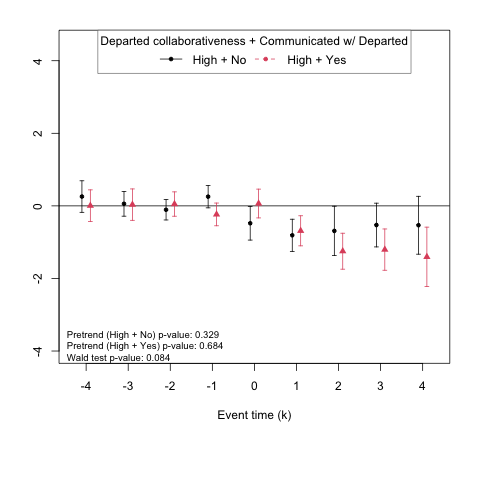
\includegraphics[width=\textwidth]{temp/output/collab/cs_norm_prs_opened_dept_never_comm_predep_High.png}
    \end{minipage}
    \hfill
    \label{fig:prs_opened_comm_ext_marg_low}
    \centering
        \begin{minipage}[b]{0.49\textwidth}
        \centering
        \subcaption{Less collaborative } \label{fig:predep_prs_opened_low_collab_comm_ext_marg}
        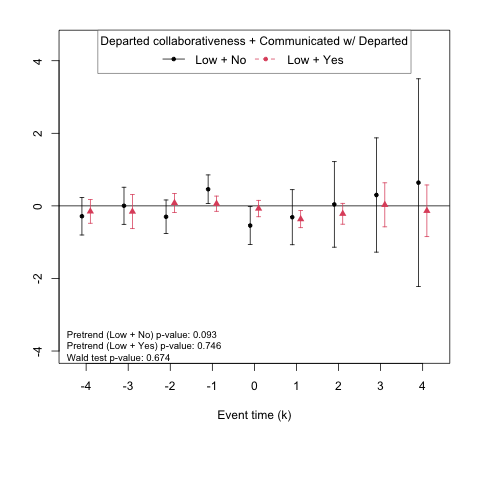
\includegraphics[width=\textwidth]{temp/output/collab/cs_norm_prs_opened_dept_never_comm_predep_Low.png}
    \end{minipage}
    
  \begin{minipage}{1\textwidth}
    \textbf{Figure notes:} 
    Following Callaway and Sant’Anna (2021), I estimate event-study coefficients accompanied by 95\% simultaneous confidence bands. For each plot with event study estimates from two subsamples, I report three Wald-test p-values: one for the pretrend test in the first subsample, one for the pretrend test in the second subsample (both from Equation \ref{eq:wald_test_pretrends} in Section \ref{sec:main_method}), and one for the difference in treatment effects across subsamples (Equation \ref{eq:wald_test} in Section \ref{sec:att_subset}). 
    Panel~\subref{fig:predep_prs_opened_high_collab_comm_ext_marg} replaces the standardized outcome’s total pull request count with that of two different member subsets: members who had ever \textbf{communicated with the departed} and members who had \textbf{never communicated with the departed} prior to estimation (as defined in Section~\ref{sec:contr_subset}) and conditions on organizations with highly collaborative departed members.
    Panel~\subref{fig:predep_prs_opened_low_collab_comm_ext_marg} is the analog of Panel~\subref{fig:predep_prs_opened_high_collab_comm_ext_marg} for less collaborative departed members.  
  \end{minipage}
  

\end{figure}
